% You can have as much text here as you want. The main body must be at most $8$ pages long.
% For the final version, one more page can be added.
% If you want, you can use an appendix like this one.  

% The $\mathtt{\backslash onecolumn}$ command above can be kept in place if you prefer a one-column appendix, or can be removed if you prefer a two-column appendix.  Apart from this possible change, the style (font size, spacing, margins, page numbering, etc.) should be kept the same as the main body.

% \section{Notations} \label{sec:notation}

\newpage
\appendix
\onecolumn
\section*{Appendix}
\section{Additional Discussion} \label{appendex:discussion}

% \subsection{Usage of LLMs Statement}
% We used Grammarly (\url{https://www.grammarly.com/}) to identify and correct grammatical errors. All revisions were manually reviewed by the authors to ensure the original meaning remained unchanged.
\subsection{Broader Application}
\label{appendex: impact}
% In this paper, we introduce a non-greedy longitudinal active feature acquisition method, \texttt{\OurMethod}, which could aid the decision-making process in real-world applications such as healthcare by selectively acquiring essential examinations; thus minimizing patient burden (e.g., time and costs) through personalized and timely intervention, as in any ML system, using \texttt{\OurMethod} should involve thorough/robust evaluations and supervision by medical professionals to prevent any potential negative impact.
We acknowledge that our experiments focus on the healthcare domain, an important application area; however, our method is not specific to any domain. Similar resource-constrained scenarios also exist in other domains, such as in energy-aware audio recognition \citep{monjur2023soundsieve} or IoT devices \citep{dunkels2011powertrace}. In fact, our AFA formulation has applications across a myriad of domains, including robotics (acquisition of sensors with resource constraints), education (acquisition of different exam types without overburdening students), and beyond.

\subsection{Assumptions \& Limitations}
\label{appendex:Limitations}
Like traditional AFA methods and RL-based baselines, \texttt{\OurMethod} assumes that the problem has a finite horizon with a limited number of time steps. Additionally, we acknowledge that, similar to other baselines presented in this paper, the performance of \texttt{\OurMethod} is sensitive to the data quality. In particular, poor label annotation in real-world clinical datasets can degrade the accuracy. However, extending to an infinite-horizon setting and mitigating the sensitivity to the data quality are beyond the scope of this paper. We will leave these challenges for future work. 



\subsection{Time Complexity}
\label{appendex:Time}
With a total of time steps $L$ and a total number of features $M$, the time complexity is $O(ML^2)$ for RL baselines (RAS, AS, ASAC), and $O(M^2L^2)$ for DiFA and DIME. For neural estimator \texttt{NOCT-Amortized}, with a random subset search of size $|\mathcal{O}|$ (i.e., number of candidate plans), the time complexity is $O(ML^2|\mathcal{O}|)$. However, if one wants to incorporate the instance-based estimator \texttt{NOCT-Contrastive} with the number of training points $n$, the time complexity is $O(nML^2|\mathcal{O}|)$, where a naive similarity-based retrieval over the $n$ training embeddings costs $O(nML)$. Note that both estimators can further parallelize the $|\mathcal{O}|$ subsets across independent workers.

\subsection{Proof of Theorem 3.1: $-\mathrm{NOCT}$ Lower Bounds the Optimal Longitudinal AFA MDP Value}
\label{appendex:theorem}
% \textbf{Theorem 1.} \emph{The value of the optimal longitudinal AFA MDP policy is lower bounded by \texttt{\OurMethod}}.

\textbf{Theorem 3.1.} \emph{(Informal) $-\mathrm{NOCT}$ lower bounds the value of the optimal longitudinal AFA MDP policy}

\uline{Problem Setup.} For any observations $(x_o, o, t)$, let the set of remaining feature-time pairs that are still available after time $t$ be:
\begin{equation*}
\mathcal{V}_{>t} = \{(m, t') \mid m \in \{1, \ldots, M\}, \, t' \in \{t+1, \ldots, L\}\}.
\end{equation*}
To follow the convention of reinforcement learning literature, we redefine the objective NOCT (Eq.~(\ref{eq:obj})) as maximization instead of minimization without loss of generality. For notational convenience, we write $\texttt{NOCT-MAX}^s_t(x_o)\equiv \texttt{NOCT-MAX}^s_t(x_o,o)$, since $x_o$ is indexed by the observation set $o$. That is, for any partial observation $(x_o,o,t)$, we define $\texttt{NOCT-MAX}^s_t(x_o)$ as:

\begin{equation*}
\texttt{NOCT-MAX}_t^s(x_o) := \max_{\substack{v\subseteq \mathcal{V}_{>t} \\ \text{s.t } \mid\text{rounds}(v) \mid \leq s} }
\Bigl[ - \mathbb{E}_{y_{t+1:L}, x_v \mid {x}_{o} }[\ell (x_o \cup x_v, y, t)] - \alpha \!\!\!\! \sum_{(m, t') \in v} \!\!\!\! c^m \Bigr],
\end{equation*} 
where $s \in \mathbb{N}$ represents the maximum number of possible future acquisition rounds, and let $\text{rounds}(v) := \{ t' \mid  \exists m \in \{1,\ldots,M\}:(m, t') \in v \}$. We then define 
\begin{equation*}
V_t^0(x_o) := -\mathbb{E}_{y_{t+1:L}\mid x_o}[\ell(x_o, y, t)] 
\end{equation*}
and 

\begin{align}
\label{eq:value_func}
V_t^s(x_o) &:=  \max \Bigl\{V_t^0 (x_o), \max_{\substack{t' \in \{t+1, ..., L\} \\ a_{t'} \in \{0,1\}^M}} \Bigl[ -\alpha \sum_{m} a_{t',m}c^m +\mathbb{E}_{x_{a_{t'}}\mid x_o} [ V^{s-1}_{t'} (x_{o \cup a_{t'}} ) ]  \Bigr] \Bigr\}.
% &\geq 
\end{align}

We see that $V^{0}_{t}$ is the expected negative cumulative loss when we immediately terminate at $t$, and we predict the future labels using only what we have acquired so far, $x_o$. Thus, $V^{s}_{t}$ is the value for the optimal longitudinal AFA policy, such that it either (i) terminates, returning $V_t^0$ or (ii) executes another acquisition at the future time step $t' \in (t+1,...,L)$ and acquires the feature $a_{t'}\in \{0,1\}^M$. 
%We want to note that $V_{t}^{s}(x)$ (Eq. (\ref{eq:value_func})) is monotone and non-decreasing in $s$. Hence, replacing the maximum of acquisition rounds from $L-t$ with an upper bound $s-1$ will increase the value of $V_{t}^{s}(x)$, and so the inequality in our lower bound proof below is preserved. The same argument is also applicable to $\texttt{\OurMethod}_t^s(x_o)$.

\uline{Claim.}
For every $(x_o, o, t)$ with $s \in \mathbb{N}_{\geq 0}$, we have $V_t^s(x_o) \geq \texttt{NOCT-MAX}^s_t(x_o)$.

\uline{Proof.}

\emph{Base case $s=0$.} Since there is no further action, both the MDP agent and \texttt{NOCT-MAX} terminate:
\begin{equation*}
V_{t}^0(x_o) =  -\mathbb{E}_{y_{t+1:L}\mid x_o}[\ell (x_o, y, t)] = \texttt{NOCT-MAX}^0_t(x_o).
\end{equation*}
\emph{Inductive hypothesis.} Assume for $s-1 \geq 0$, we have: 
\begin{equation}
V_{t'}^{s-1}(x) \geq \texttt{NOCT-MAX}^{s-1}_{t'}(x) \quad \forall (x,t').
\tag{IH}
\end{equation}
\emph{Inductive step.} We fix $(x_o, t)$ and see that: 
\begin{align*}
&V_t^s(x_o) 
\\ &= \max \Bigl\{V_t^0(x_o), \max_{\substack{t' \in \{t+1, ..., L\} \\ a_{t'} \in \{0,1\}^M}} \Bigl[ -\alpha \sum_{m} a_{t',m}c^m + \mathbb{E}_{x_{a_{t'}}\mid x_o} [V^{s-1}_{t'} (x_{o \cup a_{t'}} )]  \Bigr] \Bigr\}
\\
& \!\!\overset{(\text{IH})}{\geq} \max  \Bigl\{V_t^0(x_o), \max_{\substack{t' \in \{t+1, ..., L\} \\ a_{t'} \in \{0,1\}^M}} \Bigl[ -\alpha \sum_{m} a_{t',m}c^m + \mathbb{E}_{x_{a_{t'}}\mid x_o} [\texttt{NOCT-MAX}^{s-1}_{t'} (x_{o \cup a_{t'}} )]  \Bigr] \Bigr\}
\\
&= \max  \Bigl\{V_t^0(x_o), \\ &\max_{\substack{t' \in \{t+1, ..., L\} \\ a_{t'} \in \{0,1\}^M}} \Bigl[ -\alpha \sum_{m} a_{t',m}c^m + \mathbb{E}_{x_{a_{t'}}\mid x_o} \Bigl[\!\!\!\!\max_{\substack{v'\subseteq \mathcal{V}_{>t'} \\ \text{s.t } \mid\text{rounds}(v') \mid \leq s-1} }
\!\!\!\!\!\!\!\!\!\!\!\Bigl( - \mathbb{E}_{y_{t'+1:L}, x_{v'} \mid {x}_{o}, x_{a_{t'}} }[\ell (x_o \cup x_{a_{t'}}\cup x_{v'}, y, t')] - \alpha \!\!\!\!\!\! \sum_{(m, t'') \in v'} \!\!\!\!\!\!c^m \Bigr)\Bigr]  \Bigr] \Bigr\}
\\
&\overset{*}\geq \max  \Bigl\{V_t^0(x_o), \\
&\max_{\substack{t' \in \{t+1, ..., L\} \\ a_{t'} \in \{0,1\}^M}} \max_{\substack{v'\subseteq \mathcal{V}_{>t'} \\ \text{s.t } \mid\text{rounds}(v') \mid \leq s-1} }   \left [
- \mathbb{E}_{y_{t'+1:L}, x_{v'}, x_{a_{t'}}\mid {x}_{o} }[\ell (x_o \cup x_{a_{t'}}\cup x_{v'}, y, t')] - \alpha  \Bigl(\sum_{(m, t'') \in v'} \!\!\!\! c^m + \sum_{m} a_{t',m}c^m \Bigr ) \Bigr\} \right ]
\\
&= \max\Bigl\{V_t^0(x_o), \max_{\substack{v \in \mathcal{V}_{>t} \\ \text{s.t } |\text{rounds}(v)| \le s} } 
[ - \mathbb{E}_{y_{t+1:L}, x_v \mid {x}_{o} }[\ell (x_o \cup x_v, y, t)] - \alpha \!\!\!\! \sum_{(m, t'') \in v} \!\!\!\! c^m]\Bigr\}
\\
&= \texttt{NOCT-MAX}^{s}_{t} (x_o).
\end{align*}

where * follows from:
\[
\begin{aligned}
&\begin{array}{r}
\forall v' \in \Omega, x_{a_{t'}}, \max\limits_{v \in \Omega} \mathcal{L}\left(x_{a_{t'}}, v\right) \geq \mathcal{L}\left(x_{a_{t'}}, v'\right) \quad \Longrightarrow \\[0.8em]
\forall v'\in \Omega, \mathbb{E}_{x_{a_{t'}} \mid x_o}\left[\max\limits _{v \in \Omega} \mathcal{L}\left(x_{a_{t'}}, v\right)\right] \geq \mathbb{E}_{x_{a_{t'}} \mid x_o}\left[\mathcal{L}\left(x_{a_{t'}}, v'\right)\right] \Longrightarrow \\[0.8em]
\mathbb{E}_{x_{a_{t'}} \mid x_o}\left[\max\limits _{v \in \Omega} \mathcal{L}\left(x_{a_{t'}}, v\right)\right] \geq \max\limits _{v \in \Omega} \mathbb{E}_{x_{a_{t'}} \mid x_o}\left[\mathcal{L}\left(x_{a_{t'}}, v\right)\right]
\end{array}
\end{aligned}
\]
for $\Omega :=\Bigl\{v\subseteq\mathcal V_{>t'}\;\bigm|\; |\text{rounds}(v)|\le s-1\Bigr\}$ and 
\[
\mathcal{L} (x_{a_{t'}}, v) := 
- \mathbb{E}_{y_{t+1:L}, x_{v'} \mid {x}_{o}, x_{a_{t'}} }[\ell (x_o \cup x_{a_{t'}}\cup x_{v'}, y, t')] - \alpha  \left(\sum_{(m, t'') \in v'} \!\!\!\! c^m + \sum_{m} a_{t',m}c^m \right ).
\]

Note that one
may recover the non-cardinality constrained problem by considering large enough $s$, yielding a lower bound on the longitudinal AFA MDP.

\subsection{Proof of Proposition 3.2: Dynamic Replanning is Never Worse}
\label{appendex:proposition1}
\textbf{Proposition 3.2.} \emph{(Informal) Replanning after each acquisition is never worse (in terms of the $\mathrm{NOCT}$ objective) than committing to the original plan’s remainder.}


\uline{Problem Setup.} Fix any observation state $(x_o,o,t)$ and let the set of all feature-time pairs that are available be:  $\mathcal{V}_{>t} := \{(m,t') : t < t' \le L\}$.
Let the current plan be
\[
u(x_o,o) \in \arg\min_{v \subseteq \mathcal{V}_{>t}} \mathrm{NOCT}(x_o,o,v).
\]
If $u(x_o,o)=\emptyset$, then we stop the acquisition and the claim is trivial. Otherwise, we define the next acquisition time $t_\text{next}$ and the set of acquisitions $a_{t_{\text{next}}}$ at time $t_{\text{next}}$ be:
\begin{align*}
t_{\text{next}} := \min\{t' : (m,t') \in u(x_o,o)\}, 
\qquad
a_{t_{\text{next}}} := \{(m,t_{\text{next}})\in u(x_o,o)\}.
\end{align*}
After observing $x_{a_{t_{\text{next}}}}$, we update the current observed features $o':=o\cup a_{t_{\text{next}}}$ and
$x_{o'}:=x_o\cup x_{a_{t_{\text{next}}}}$,
and define the remainder of the original plan after $t_{\text{next}}$:
\begin{align*}
\tilde u := \{(m,\tau)\in u(x_o,o) : \tau > t_{\text{next}}\} \subseteq \mathcal{V}_{>t_{\text{next}}}.
\end{align*}

\textit{$\mathrm{NOCT}$ of the original strategy}: We can decompose $\mathrm{NOCT}$ by splitting the
loss sum at $t_{\text{next}}$ and splitting the costs into those at $t_{\text{next}}$
and those after $t_{\text{next}}$. This yields:
\begin{align}
\mathrm{NOCT}(x_o,o,u(x_o,o))
&=
\mathbb{E}_{y_{t+1:t_{\text{next}}},\,x_{a_{t_{\text{next}}}} \mid x_o}
\Bigg[
\sum_{k=t+1}^{t_{\text{next}}}
\mathrm{CE}\!\Big(\hat y_k\big(x_o \cup x_{u(x_o,o)^{t+1:k}}\big),\,y_k\Big)
\Bigg]
\;+\;\alpha \sum_{(m,t_{\text{next}})\in a_{t_{\text{next}}}} c_m
\nonumber\\
&\qquad\qquad
+\;\mathbb{E}_{x_{a_{t_{\text{next}}}} \mid x_o}\Big[\,\mathrm{NOCT}(x'_o,o',\tilde u)\,\Big],
\label{eq:noct_commit}
\end{align}
where $u(x_o,o)^{t+1:k}$ denotes the subset of original plan $u(x_o,o)$ restricted to times
$t+1,\ldots,k$.

\textit{$\mathrm{NOCT}$ of the replanning strategy}: Let $\mathcal{R}(x_o,o,t)$ denote the expected $\mathrm{NOCT}$ objective by the replanning strategy that repeats:
(i) compute $u(\cdot)$ via Eq.~(\ref{eq:nocta}), (ii) execute its next acquisition $(t_{\text{next}},a_{t_{\text{next}}})$,
 (iii) update $(x_o,o,t)$, and (iv) repeat step (i) (Alg.~\ref{alg:nocta}).
With this definition, $\mathcal{R}(x_o,o,t)$ is the recursion defined as:
\begin{align}
\mathcal{R}(x_o,o,t)
&=
\mathbb{E}_{y_{t+1:t_{\text{next}}},\,x_{a_{t_{\text{next}}}} \mid x_o}
\Bigg[
\sum_{k=t+1}^{t_{\text{next}}}
\mathrm{CE}\!\Big(\hat y_k\big(x_o \cup x_{u(x_o,o)^{t+1:k}}\big),\,y_k\Big)
\Bigg]
\;+\;\alpha \sum_{(m,t_{\text{next}})\in a_{t_{\text{next}}}} c_m
\nonumber\\
&\qquad\qquad
+\;\mathbb{E}_{x_{a_{t_{\text{next}}}} \mid x_o}\Big[\,\mathcal{R}(x'_o,o',t_{\text{next}})\,\Big].
\label{eq:noct_replan}
\end{align}
Please note that the first two terms in Eq. \eqref{eq:noct_replan} match with those in Eq. \eqref{eq:noct_commit} because both
strategies execute the same first acquisition at $t_{\text{next}}$ and thus
make identical predictions up to $t_{\text{next}}$; \textit{the only difference is the continuation} (we will utilize this fact later in the proof).

\uline{Claim.} For all $(x_o,o,t)$, $\mathcal{R}(x_o,o,t)\;\le\;\mathrm{NOCT}(x_o,o,u(x_o,o)).$


\uline{Proof.} 

We will prove this with backward induction. 

\emph{Base case.} The base case is $t=L$ (i.e., $\mathcal{V}_{>t}=\emptyset$), where both strategies
terminate immediately and are equal.


\emph{Inductive hypothesis.} Assume that for every state $(\bar x_o,\bar o,\bar t)$
with smaller remaining horizon (i.e., $L-\bar t < L-t$), we have:
\begin{equation}
\mathcal{R}(\bar x_o,\bar o,\bar t)\ \le\ \mathrm{NOCT}(\bar x_o,\bar o, u(\bar x_o,\bar o)).
\label{eq:IHproposition}
\end{equation}



\emph{Inductive step.} We fix $(x_o,o,t)$ with $u(x_o,o)\neq\emptyset$ and the corresponding
$t_{\text{next}},a_{t_{\text{next}}},(x'_o,o')$ defined above. Since $t_{\text{next}} > t$,
we have $L-t_{\text{next}} < L-t$, so the induction hypothesis Eq. (\ref{eq:IHproposition}) applies at
$(x'_o,o',t_{\text{next}})$:
\begin{align}
\mathcal{R}(x'_o,o',t_{\text{next}})\;\le\;\mathrm{NOCT}(x'_o,o',u(x'_o,o')).
\label{eq:optimal1}
\end{align}
Moreover, by optimality of $u(x'_o,o')$ at state $(x'_o,o',t_{\text{next}})$ and $\tilde u \subseteq \mathcal{V}_{>t_{\text{next}}}$ (as the construction 
of $\tilde u$), we have:
\begin{align}
\mathrm{NOCT}(x'_o,o',u(x'_o,o')) \;=\; \min_{v\subseteq \mathcal{V}_{>t_{\text{next}}}}
\mathrm{NOCT}(x'_o,o',v)
\;\le\; \mathrm{NOCT}(x'_o,o',\tilde u).
\label{eq:optimal2}
\end{align}
Combining Eq.~(\ref{eq:optimal1}) and Eq.~(\ref{eq:optimal2}) gives, for every realized
$x_{a_{t_{\text{next}}}}$,
\begin{align*}    
\mathcal{R}(x'_o,o',t_{\text{next}})\;\le\;\mathrm{NOCT}(x'_o,o',\tilde u).
\end{align*}

Taking the expectation over $\mathbb{E}_{x_{a_{t_{\text{next}}}} \mid x_o}$ preserves the inequality. Finally, substituting this bound into the decompositions of Eq.~(\ref{eq:noct_commit}) and Eq.~(\ref{eq:noct_replan}) (which share identical prefix terms up to $t_{\text{next}}$) yields:
\begin{align*}
\mathcal{R}(x_o,o,t)\;\le\;\mathrm{NOCT}(x_o,o,u(x_o,o)).
\end{align*}
Hence, the results follow. 
% \subsection{Proof of Proposition 2: Robustness to NOCT Estimation Error}
% \label{appendex:regret}
% \textbf{Lemma 1.} \emph{$\mathrm{NOCT}(x_o,o,\hat u)\; \le\;\mathrm{NOCT}(x_o,o,u)\; + \;2\varepsilon.
% $}

% \uline{Problem Setup.} With any obeservation $(x_o,o,t)$ and let $\mathrm{NOCT}$ be the oracle and $\widehat{\mathrm{NOCT}}$ be the estimator of $\mathrm{NOCT}$. We have the oracle plan as 

% \[
% u(x_o,o)\in \arg\min_{v\subseteq V_{>t}} \mathrm{NOCT}(x_o,o,v),
% \]
% and the estimated plan as
% \[
% \hat{u}(x_o,o)\in \arg\min_{v\subseteq V_{>t}} \widehat{\mathrm{NOCT}}(x_o,o,v). 
% \]
% Let $s$ be the maximum number of remaining acquisition rounds (as in Appx. \ref{appendex:theorem}).

% \uline{Claim.} 
% Assume a uniform estimation error bound with observation $(x_o,o,t)$:
% \[
% \sup_{v\subseteq V_{>t}}\big|\widehat{\mathrm{NOCT}}(x_o,o,v)-\mathrm{NOCT}(x_o,o,v)\big |\; \le \; \varepsilon.
% \]
% Then the plan chosen by the estimator satisfies
% \[
% \mathrm{NOCT}(x_o,o,\hat u)\; \le\;\mathrm{NOCT}(x_o,o,u)\; + \;2\varepsilon.
% \]


% \uline{Proof.} 
% Since $\hat{u}$ minimizes $\widehat{\mathrm{NOCT}}$, we have:
% \[
% \widehat{\mathrm{NOCT}}(x_o,o,\hat u)\; \le\; \widehat{\mathrm{NOCT}}(x_o,o,u).
% \]
% Using the uniform deviation bound twice,
% \[
% \mathrm{NOCT}(x_o,o,\hat u)
% \le
% \widehat{\mathrm{NOCT}}(x_o,o,\hat u)+\varepsilon
% \le
% \widehat{\mathrm{NOCT}}(x_o,o,u)+\varepsilon
% \le
% \mathrm{NOCT}(x_o,o,u)+2\varepsilon.
% \]

% \textbf{Proposition 2.} \emph{(Informal) If $\widehat{\mathrm{NOCT}}$ estimates $\mathrm{NOCT}$ within $\varepsilon$ error at each replanning round, then the resulting policy is at most $O(s\varepsilon)$ worse than oracle-\texttt{\OurMethod}, where $s$ is the maximum number of remaining acquisition rounds.} 

% \uline{Problem Setup.}
% With any observation $(x_o,o,t)$ and the plan $v\subseteq V_{>t}$. Let $u_r\in\arg\min_v \mathrm{NOCT}(x_o,o,v)$ denote the oracle plan at replanning round $r$ and
% $\hat u_r\in\arg\min_v \widehat{\mathrm{NOCT}}(x_o,o,v)$ the plan using the estimator. After $r-1$ acquisition round, let $o^{(r)} := o \cup \bigcup_{j=1}^{r-1} a_{t_j}$ be the acquired feature-time pairs, and
% let $x_o^{(r)} := x_o \cup \bigcup_{j=1}^{r-1} x_{a_{t_j}}$ be the corresponding observed values.


% \uline{Claim.}  Let $\varepsilon_r$ denote the uniform $\mathrm{NOCT}$ estimation error at round $r$, i.e.,
% \begin{equation}
% \label{eq:uniform_regret}
% \sup_{v\subseteq V_{>t}}\big|\widehat{\mathrm{NOCT}}(x_o,o,v)-\mathrm{NOCT}(x_o,o,v)\big |\; \le \; \varepsilon_r.
% \end{equation}
% Then, following Lemma 1, the per-round suboptimality satisfies
% \begin{equation}
% \label{eq:per_round_regret}
% \mathrm{NOCT}(x_o,o,\hat u_r) \;\le\; \mathrm{NOCT}(x_o,o,u_r) + 2\varepsilon_r .
% \end{equation}
% If we follow \texttt{\OurMethod} Algorithm (\ref{alg:nocta}) to replan for at most $s$ acquisition rounds (as in Appx. \ref{appendex:theorem}), then
% \begin{equation}
% \label{eq:cum_regret}
% \sum_{r=1}^{R}
% \Big(
% \mathrm{NOCT}(x_o^{(r)},o^{(r)},\hat u_r)
% -
% \mathrm{NOCT}(x_o^{(r)},o^{(r)},u_r)
% \Big)
% \;\le\;
% 2\sum_{r=1}^{s}\varepsilon_r
% \;\le\;
% 2s\varepsilon
% \qquad \text{for  } R\le s \text{ and } \varepsilon_r \leq \varepsilon.
% \end{equation}

% \uline{Proof.}
% With a fixed round $r$ and its state $(x_o,o,t)$. Since $\hat u_r$ minimizes $\widehat{\mathrm{NOCT}}$,
% $\widehat{\mathrm{NOCT}}(x_o,o,\hat u_r)\le \widehat{\mathrm{NOCT}}(x_o,o,u_r)$.
% Applying~\eqref{eq:uniform_regret} to both plans yields
% \[
% \mathrm{NOCT}(x_o,o,\hat u_r)
% \le \widehat{\mathrm{NOCT}}(x_o,o,\hat u_r)+\varepsilon_r
% \le \widehat{\mathrm{NOCT}}(x_o,o,u_r)+\varepsilon_r
% \le \mathrm{NOCT}(x_o,o,u_r)+2\varepsilon_r,
% \]
% which shows~\eqref{eq:per_round_regret}. Summing over at most $R\le s$ replanning rounds gives~\eqref{eq:cum_regret}. Hence, the results follow.

\subsection{Future-Candidate Distribution $\zeta_o$.}
\label{appendex:future_dist}
In this section, we formally introduce the future-candidate distribution $\zeta_o$. For any partially observed features $x_o$ at time $t$ and the corresponding labels $y$ of the training dataset $\mathcal{D}$, we identify the top-$\kappa$ candidate subsets $v_1, \ldots, v_\kappa \subseteq \mathcal{V}_{>t}
= \{(m, t') \mid m \in \{1, \ldots, M\}, \, t' \in \{t+1, \ldots, L\}\}$, in ascending order of the plug-in objective $\mathrm{NOCT}_{\mathrm{pl}}(x_o, o, v_l)$ (Eq.~(\ref{eq:plugobj})).
% we identify the top-$\kappa$ candidate subsets $v_1, \ldots, v_\kappa \subseteq  \mathcal{V}_{>t} = \{(m, t') \mid m \in \{1, \ldots, M\}, \, t' \in \{t+1, \ldots, L\}\}$, in ascending order of:
% % {\small
% \begin{equation}
%  r_{l} = \ell (x_o \cup x_{v_l}, y, t) + \alpha \!\!\!\! \sum_{(m, t') \in {v_l}} \!\!\!\! c^m. 
% \label{eq:embedding}
% \end{equation}
$\mathrm{NOCT}_{\mathrm{pl}}(x_o, o, v_l)$ quantifies the accuracy-cost tradeoff for candidate $v_l$, and we have access to $x_{v_l}$ during training since $x_{v_l}$ is from the training set. Now, each candidate $v_l$ induces a uniform distribution $\nu_{v_l}$ over its selected feature-time pairs (and termination), defined as $\nu_{v_l}(m,t') = \tfrac{1}{|v_l|}$ if $(m,t') \in v_l$ and $0$ otherwise. Intuitively, $\nu_{v_l}$ spreads equal probability mass over all acquisitions in the future candidate plan $v_l$. Note that in the case that $v_l$ contains no further acquisition, $\nu_{v_l}(\varnothing) = 1$ (and if $v_l$ is not empty $\nu_{v_l}(\varnothing) = 0$). The future-candidate distribution $\zeta_o$ for observed features $x_o$ is the weighted sum of $\nu_{v_l}$ as  
\begin{equation}
\zeta_o = \sum_{l=1}^{\kappa} w_l \ \nu_{v_l}
\label{eq:prob}
\end{equation}

where $w_l = \frac{\exp\!\big(-\mathrm{NOCT}_{\mathrm{pl}}(x_o,o,v_l)\big)}{\sum_{k=1}^\kappa \exp\!\big(-\mathrm{NOCT}_{\mathrm{pl}}(x_o,o,v_k)\big)}$. Intuitively, given a partially observed feature $x_o$, $\zeta_o$ indicates how likely each feature at each timestep (and the termination) is chosen by weighting their accuracy-cost
tradeoff. For each training sample $(x_i, y_i) \in \mathcal{D}$, we construct $\zeta_{i,o}$ accordingly.


\subsection{Sensitivity Analysis}
\label{appendex:sensitivity}
In this section, we provide further explanations of hyperparameters and how they affect performance. Overall, we find that our proposed method is robust to different settings, indicating that our method can be applied readily without excessive fine-tuning.


% \item $\alpha$: this is to balance the tradeoff between the accumulated loss (e.g., cross-entropy) and the acquisition cost for future features. A larger $\alpha$ will emphasize more on minimizing the cost, which leads to a lower number of acquisitions, and a smaller $\alpha$ emphasizes reducing the prediction loss, which leads to a higher number of acquisitions.

$|\mathcal{O}|$: this specifies the size of the candidate subset in our search. As $|\mathcal{O}|$ increases, \texttt{\OurMethod} can explore a broader set of potential acquisition plans. As seen in Tab.~\ref{tab:subset_size_np} and  Tab.~\ref{tab:subset_size_p}, both estimators \texttt{NOCT-Contrastive} and \texttt{NOCT-Amortized} exhibit clear diminishing returns once $|\mathcal{O}|$ exceeds 1000.

$\kappa$: this controls how many top candidate subsets are aggregated to form the future acquisition distribution Eq.~(\ref{eq:prob}). Please refer to Tab.~\ref{tab:kappa} for different settings. %As shown in Table~\ref{tab:kappa} below, $\kappa = 5$ performs better at a lower cost.

$K$: this controls how many retrieved training samples in the learned embedding space are used to estimate future acquisition gains (Eq.~\ref{eq:noctanp}). Small $K$ can yield high-variance estimates due to limited support, while large $K$ may include less similar samples. See Tab.~\ref{tab:neighbors} for different settings.
% Through our ablation in Table~\ref{tab:neighbors} below, $K = 5$ performs comparably well at a reasonable cost.


$\beta$: this controls the sensitivity that translates Jessen-Shannon divergence into a similarity score (Eq.~\ref{eq:js}). A larger $\beta$ will penalize divergences more strongly, while a smaller $\beta$ will be more lenient. Please refer to Tab.~\ref{tab:beta} for different settings. %As shown in Table~\ref{tab:beta} below, $\beta = 1$ performs comparably well at a reasonable cost.

$\gamma$: this determines the margin in the contrastive loss, making sure that dissimilar embeddings are pushed far apart (Eq.~\ref{eq:ebmedding}). If $\gamma$ is too small, the embedding network might not push dissimilar pairs far enough, and if $\gamma$ is too large, it might push moderately different samples by a large distance. Please refer to Tab.~\ref{tab:gamma} for different settings.%As we can see in Table~\ref{tab:gamma} below: $\gamma = 1$ performs better at a lower cost.

\smallskip
\begin{table}[H]
\centering
\caption{Ablation on the subset size $|\mathcal{O}|$ for \texttt{NOCT-Contrastive} used in the synthetic dataset}
\label{tab:subset_size_np}
\begin{tabular}{ccc}
\toprule
$|\mathcal{O}|$ & Accuracy & Cost \\
\midrule
$100$    & $0.843 \pm 0.001$ & $13.252 \pm 0.044$ \\
$1000$  & $0.855\pm0.002$ & $11.315\pm0.012$  \\ 
$5000$  & $0.857 \pm 0.001$ & $12.046 \pm 0.021$ \\
$10000$ & $0.857 \pm 0.002$ & $11.945 \pm 0.012$ \\
\bottomrule
\end{tabular}
\end{table}
\smallskip

\begin{table}[H]
    \centering
    \caption{Ablation on the subset size $|\mathcal{O}|$ for \texttt{NOCT-Amortized} used in the synthetic dataset}
    \label{tab:subset_size_p}
    \begin{tabular}{ccc}
        \toprule
        $|\mathcal{O}|$ & Accuracy & Cost \\
        \midrule
        $100$   & $0.651 \pm 0.010$ & $11.401 \pm 0.040$ \\
        $1000$  & $0.666\pm0.006$ & $11.555\pm0.087$ \\
        $5000$  & $0.670 \pm 0.016$ & $11.430 \pm 0.115$ \\
        $10000$ & $0.664 \pm 0.017$ & $11.419 \pm 0.150$ \\
        \bottomrule
    \end{tabular}
\end{table}

\smallskip


\begin{table}[H]
    \centering
    \caption{Ablation on the number of retrieved instances $K$ on the synthetic dataset.}
    \label{tab:neighbors}
    \begin{tabular}{ccc}
        \toprule
        $K$ & Accuracy & Cost \\
        \midrule
        $5$& $0.815\pm0.005$ & $9.471\pm0.033$ \\
        $10$ & $0.801 \pm 0.003$ & $9.489 \pm 0.006$ \\
        $25$ & $0.816 \pm 0.001$ & $9.512 \pm 0.006$ \\
        \bottomrule
    \end{tabular}
\end{table}

\smallskip
\begin{table}[H]
    \centering
    \caption{Ablation on the number of top candidate subset $\kappa$ used in the synthetic dataset}
    \label{tab:kappa}
    \begin{tabular}{ccc}
        \toprule
        $\kappa$ & Accuracy & Cost \\
        \midrule
        $5$& $0.815\pm0.005$ & $9.471\pm0.033$ \\
        $10$ & $0.814 \pm 0.001$ & $9.618 \pm 0.022$\\
        $25$ & $0.811 \pm 0.002$ & $9.564 \pm 0.067$ \\

        \bottomrule
    \end{tabular}
\end{table}
\smallskip

\begin{table}[H]
    \centering
    \caption{Ablation on the scaling in similarity function $\beta$ used in the synthetic dataset}
    \label{tab:beta}
    \begin{tabular}{ccc}
        \toprule
        $\beta$ & Accuracy & Cost \\
        \midrule
        $0.5$ & $0.810 \pm 0.002$ & $9.660 \pm 0.054$ \\
        $1$   & $0.815\pm0.005$   & $9.471\pm0.033$ \\
        $2$   & $0.821 \pm 0.001$ & $9.592 \pm 0.022$ \\
        $5$   & $0.819 \pm 0.003$ & $9.640 \pm 0.048$ \\
        \bottomrule
    \end{tabular}
\end{table}

\smallskip

\begin{table}[H]
    \centering
    \caption{Ablation on the margin in contrastive loss $\gamma$ used in the synthetic dataset}
    \label{tab:gamma}
    \begin{tabular}{ccc}
        \toprule
        $\gamma$ & Accuracy & Cost \\
        \midrule
        $0.5$ & $0.813 \pm 0.010$& $9.592 \pm 0.035$ \\
        $1$   & $0.815\pm0.005$ & $9.471\pm0.033$ \\
        $2$   & $0.809\pm 0.005$& $9.638\pm 0.033$\\
        $5$   & $0.811\pm 0.001$& $9.688\pm 0.017$\\
        \bottomrule
    \end{tabular}
\end{table}


\section{Experimental Setup} \label{appendex:experiment_setup}
\subsection{Cost of Features} \label{sec:cost}
\textbf{Synthetic data.} Our synthetic dataset includes $2$ features, one being the digit and the other being the counter. Since both are generated through random selection, we assign an equal cost, $1$, to the two features. Upon publication, we will release the synthetic dataset. 

\textbf{ADNI.} The ADNI dataset includes $4$ features per time point, with FDG and AV45 extracted from PET scans and Hippocampus and Entorhinal extracted from MRI scans. Since PET is a more expensive diagnosis, we follow~\citet{qin2024risk} and assign a cost $1$ to FDG and AV45, and a cost $0.5$ to Hippocampus and Entorhinal. Access to ADNI data may be requested via \url{https://adni.loni.usc.edu}, and the Data Use Agreement is available at \url{https://adni.loni.usc.edu/terms-of-use/}.

\textbf{OAI.} We use a total of $27$ features for the OAI dataset, with $17$ clinical measurements, and $10$ joint space width (JSW) extracted from knee radiography. For the clinical measurements, we assign a low cost of $0.3$ to those that require minimum effort, e.g., age, sex, and race, and a slightly higher cost of $0.5$ to blood pressure and BMI calculation. For JSW, a cost of $1.0$ is assigned for the minimum JSW and $0.8$ for those measured at different positions. Access to the OAI data may be requested via \url{https://nda.nih.gov/oai/}.


\subsection{Baseline Implementation} \label{sec:baseline}
For ASAC, RAS, and AS, we use the implementation available at \url{https://github.com/yvchao/cvar_sensing}, which is under the BSD-3-Clause license. For DIME~\citep{gadgil2023estimating}, we extend the method to longitudinal by building on top of the official implementation available at \url{https://github.com/suinleelab/DIME}. The DiFA codebase is not publicly released, and researchers may request it directly from the authors.

Following~\citet{qin2024risk}, we share the same neural CDE predictor ~\citep{kidger2020neural} for ASAC, RAS, and AS. Following the authors' released code, we treat the drop rate $p$ of the auxiliary observation strategy $\pi_0$ (the same notation as in ~\citet{qin2024risk}) as a hyperparameter and sweep $p \in \{0.0, 0.3, 0.5, 0.7\}$. We select $p$ based on the outcome predictor's average accuracy over five randomly masked test sets generated by $\pi_0$. This matches the original evaluation protocol to ensure comparability and reproducibility. The selected drop rates are $p=0.3$ (Synthetic), $p=0.7$ (ADNI), $p=0.5$ (WOMAC), and $p=0.3$ (KLG).

\textbf{ASAC~\citep{yoon2019asac}.} We select the coefficient for the acquisition cost: 1) $\mu \in \{0.0015, 0.002, 0.003\}$ for the synthetic dataset, 2) $\mu \in \{0.005, 0.02\}$ for ADNI, 3) $\mu \in \{0.0012, 0.0016, 0.003\}$ for the WOMAC of OAI dataset, and 4) $\mu \in \{0.00125, 0.0015, 0.00175, 0.005\}$ for the KLG of OAI dataset. Note that we report multiple final $\mu$ because we evaluate ASAC across multiple acquisition costs.

\textbf{RAS~\citep{qin2024risk}.} For the synthetic dataset, we set the allowed acquisition interval to $(\Delta_{\min} = 0.2, \Delta_{\max} = 1.0)$ for the synthetic dataset, $(\Delta_{\min} = 0.5, \Delta_{\max} = 1.5)$ for ADNI, and $(\Delta_{\min} = 0.5, \Delta_{\max} = 4.5)$ for WOMAC and KLG. 

Moreover, for RAS we tune the diagnostic-error coefficient $\gamma^{\text{RAS}}$ on the validation set via a grid search. Specifically, we sweep $\gamma^{\text{RAS}} \in \{200,250,280,300,310,320,350,400,5000,7000,9000\}$ (Synthetic), $\{50,75,100,175,200,250,300,350,400,450\}$ (ADNI), $\{200,250,300,350,400,450,2000,3000,4500,9000\}$ (WOMAC), and $\{200,250,300,350,400,450,1200,1700\}$ (KLG), and select the best value per dataset. The final selected values are $\gamma^{\text{RAS}}\in\{5000,7000,9000\}$ (Synthetic), $\{50,75,100,175\}$ (ADNI), $\{2000,4500,9000\}$ (WOMAC), and $\{1200,1700\}$ (KLG); we report multiple final $\gamma^{\text{RAS}}$ because we evaluate RAS across multiple acquisition costs. For all datasets, we use a tail-risk quantile of $0.1$, an invalid-visit penalty of $10$, and a discount factor of $0.99$, following the authors' defaults.

\textbf{AS~\citep{qin2024risk}.} We set the minimum and maximum allowed acquisition intervals as in the RAS setting. In addition, we select fixed acquisition interval of: 1) $\tilde{\Delta} \in \{0.2, 0.4\}$ for the synthetic dataset, 2) $\tilde{\Delta} \in \{0.5, 1.0, 1.5\}$ for ADNI dataset, 3) $\tilde{\Delta} \in \{0.5, 1.5\}$ for WOMAC of OAI, and 4) $\tilde{\Delta} \in \{0.5, 1.5\}$ for KLG of OAI dataset. Note that we report multiple final $\tilde{\Delta}$ because we evaluate AS across multiple acquisition costs. 

\textbf{DIME~\citep{gadgil2023estimating}.} For this baseline, we extend the original model to the longitudinal setting, while still keeping its greedy feature acquisition strategy. 
Both the prediction network and value network of DIME share the same architecture as our \texttt{NOCT-Amortized} model, and hence we use the same training strategies. 

\textbf{DiFA~\citep{ghosh2023difa}}. Following ~\citet{ghosh2023difa}, we use a variational autoencoder with arbitrary conditioning (VAEAC) probabilistic model  \citep{ivanov2018variational} for imputation. When using the same architecture with \texttt{NOCT-Contrastive}, DiFA performs poorly. Hence, we gave DiFA an advantage and used the recommended architecture from the DiFA paper. That is, both the prediction network and the feature policy model have two fully connected layers (hidden size 128) with skip connections, dropout regularizer, and LeakyReLU activation function. 

\subsection{\texttt{\OurMethod} Implementation} \label{sec:architecture}
\textbf{Prediction Network.} We share the same MLP architecture for both \texttt{NOCT-Contrastive} and \texttt{NOCT-Amortized}. Specifically, the network consists of two hidden layers with ReLU. Each hidden layer contains $10$ units for the synthetic and ADNI datasets, and $32$ units for the WOMAC and KLG of the OAI dataset, respectively. Moreover, we apply random dropout for the input during training of the predictor.

\textbf{\texttt{NOCT-Contrastive}}. We select the accuracy-cost trade-off hyperparameter: 1) $\alpha \in \{0.002, 0.006, 0.02, 0.03\}$ for the synthetic dataset, 2) $\alpha \in \{0.003, 0.005, 0.01 \}$ for ADNI dataset, 3) $\alpha \in \{0.00075, 0.005, 0.01 \}$ for WOMAC of OAI dataset, and 4) $\alpha \in \{0.0025, 0.001, 0.006 \}$ for KLG of OAI dataset. 

For the embedding network, we use four hidden layers with ReLU. Each hidden layer contains $32$ units for the synthetic and ADNI datasets, and $64$ units for the WOMAC and KLG of the OAI dataset, respectively.


\textbf{\texttt{NOCT-Amortized}.} For the estimator $f_\theta$, we use an MLP architecture with two hidden layers and ReLU as the activation function. We use the same hidden size as the prediction network, but the number of outputs is set to be $1$ for estimating the utility of the potential subset. We set the accuracy-cost trade-off hyperparameter $\alpha$ to $5e{-}5$ for WOMAC and $5e{-}4$ for all other tasks, and the acquisition terminates by either selecting the empty set or reaching the budget.

% To stabilize training of the neural NOCT estimator ($f_\theta$) in \texttt{NOCT-Amortized} (Eq.~(\ref{eq:value_mse})), we modify the regression target in two ways: 
% 1) remove the acquisition-cost term and train $f_\theta$ to predict only the accumulated CE loss; the predicted value is defined as $\widebar{\mathrm{NOCT}}(x_o,o,v,t) \;=\; \ell(x_o \cup x_v, y, t)$. Since the cost of each subset is fixed and can be directly added during subset selection, excluding it from the prediction target simplifies the learning process without affecting the final decision; 
% 2) regress the \emph{relative} improvement over the current observations: $\Delta\ell(x_o,o,v,t)\;=\;\ell(x_o, y, t) - \bar{\ell}(x_o,o,v,t)$. This represents the potential gain from acquiring new features and implicitly normalizes the loss scale. Since $\ell (x_o, y, t)$ is a constant, this will not change the selection (i.e., through $\arg\max$), and hence remains the same objective as Eq.~(\ref{eq:obj}). 

To promote more stable training for Eq.~(\ref{eq:value_mse}) in \texttt{NOCT-Amortized}, we slightly modify the neural network estimator $f_\theta$'s target in two ways. First, instead of regressing to the full plug-in objective Eq.~(\ref{eq:plugobj}), we train the estimator $f_\theta$ to predict only the predictive-loss:
\begin{equation}
\label{eq:nocta_pl_loss_only}
\widetilde{\mathrm{NOCT}}_{\mathrm{pl}}(x_o,o,v)\;\triangleq\;\ell(x_o\cup x_v, y, t),
\end{equation}
and add $\alpha\sum_{(m,t')\in v} c^m$ explicitly when ranking candidate plans, since it depends only on $v$ (which we have access to during inference time). Second, we further reformulate the target as the gain relative to terminating with the current information:
\begin{equation}
\label{eq:delta_pl}
\Delta_{\mathrm{pl}}(x_o,o,v)\;\triangleq\;\ell(x_o, y, t)\;-\;\widetilde{\mathrm{NOCT}}_{\mathrm{pl}}(x_o,o,v).
\end{equation}
Because $\ell(x_o,y,t)$ is constant w.r.t.\ $v$ at a fixed state $(x_o,o,t)$, maximizing $\Delta_{\mathrm{pl}}$ is equivalent to minimizing $\widetilde{\mathrm{NOCT}}_{\mathrm{pl}}$ (and thus yields the same plan $u(x_o, o)$ in Eq.~(\ref{eq:nocta})). That is, the target of the neural network estimator $f_\theta$ is now $\Delta_{\mathrm{pl}}(x_o,o,v)$, and this implicitly normalizes the target scale. 


\subsection{Hardware} \label{sec:hardware}
We employed two different clusters for our experiments: (1) Intel Xeon CPU E5-2630 v4 and NVIDIA GeForce GTX 1080 for experiments, and (2) Intel Xeon Silver 4114 CPU and NVIDIA GeForce GTX 2080. We used cluster (1) for RAS, AS, ASAC, DiFA, \texttt{NOCT-Contrastive}, and cluster (2) for DIME and \texttt{NOCT-Amortized}

% \clearpage
\section{Additional Results} \label{appendex:results}
% We show the prediction result for each method under two different costs for different tasks below. We use \textbf{bold} to mark the highest performance and \underline{underline} for the second highest performance.
\subsection{ROC AUC on Real-World Datasets}
Following \citet{qin2024risk}, Fig.~\ref{fig:roc_auc} shows additional ROC AUC results on real‑world datasets across varying average acquisition budgets. Our method consistently outperforms all baselines while using a lower cost.

\begin{figure*}[h] 
  \centering
    \resizebox{0.8\textwidth}{!}{

  % ----- 1st column -------------------------------------------------
  \begin{subfigure}[t]{.32\textwidth}
    \centering
    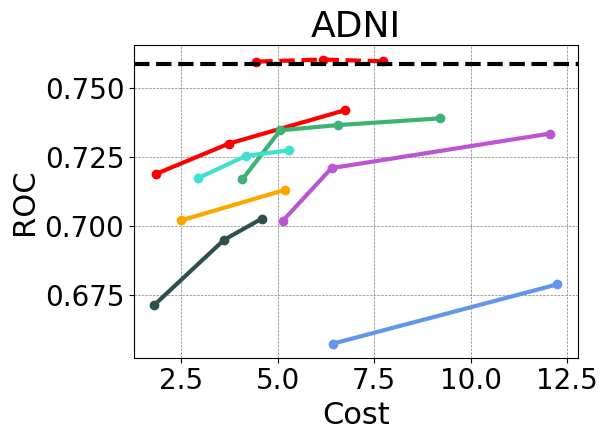
\includegraphics[width=\linewidth]{figures/adni_roc.png}
    % \caption{Synthetic}\label{fig:sub1}
  \end{subfigure}
  % ----- 2nd column -------------------------------------------------
  \begin{subfigure}[t]{.32\textwidth}
    \centering
    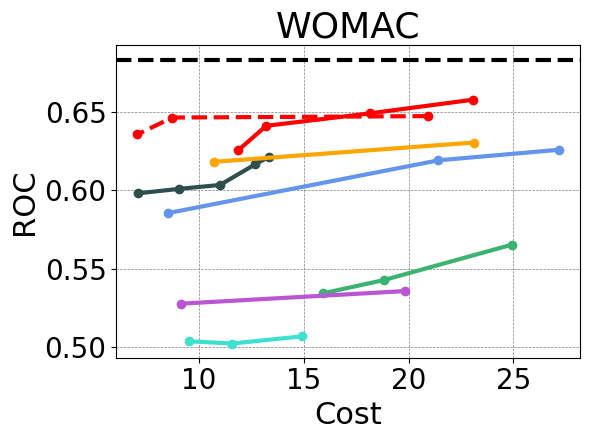
\includegraphics[width=\linewidth]{figures/womac_roc.png}
    % \caption{ADNI}\label{fig:sub2}
  \end{subfigure}
  % ----- 3rd column -------------------------------------------------
  \begin{subfigure}[t]{.32\textwidth}
    \centering
    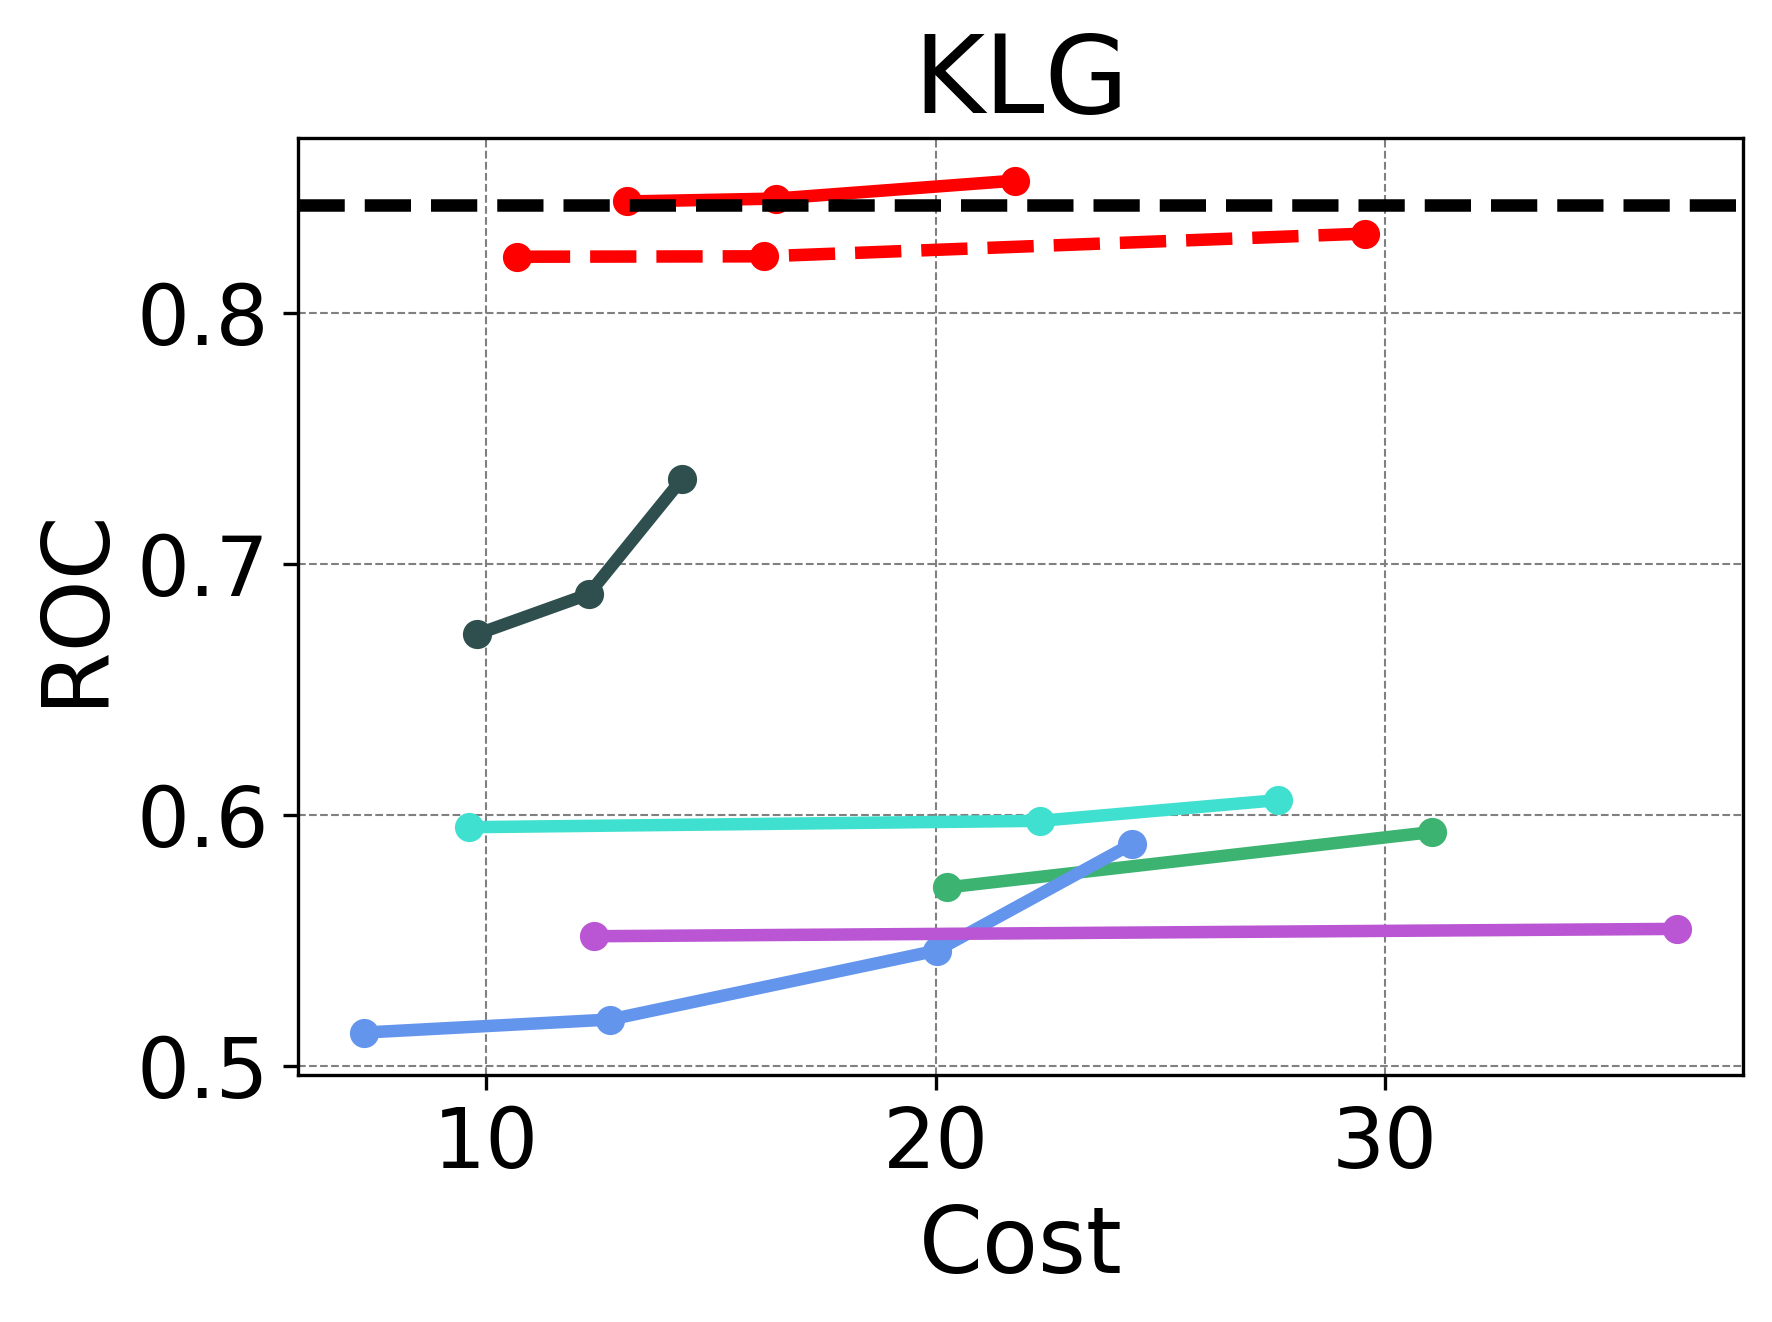
\includegraphics[width=\linewidth]{figures/klg_roc.png}
    % \caption{WOMAC}\label{fig:sub3}
  \end{subfigure}
  }
  % \par\bigskip            % vertical gap between plots and legend
  \begin{minipage}{\textwidth}
    \centering
    % trim=⟨left bottom right top⟩ clip    — remove surrounding whitespace if needed
    
\includegraphics[width=0.9\textwidth,trim=0 0 0 0,clip]{figures/legend_only.png}
  \end{minipage}
  \caption{Additional results on performance/cost of models, measured by ROC AUC across varying average acquisition budgets on real‑world datasets. Best viewed in color.}
  \label{fig:roc_auc}
\end{figure*}

\subsection{Full Results with Mean and Standard Deviation}
Tables.~\ref{tab:synthetic}, \ref{tab:adni}, \ref{tab:womac}, and \ref{tab:klg} report the mean and standard deviation for each data point presented in Figs.~\ref{fig:performance} and~\ref{fig:roc_auc}, computed over five independent runs.


\begin{table}[ht]
\captionsetup{
    % skip=10pt,
    %font=9pt,
    % labelfont=it 
}
\caption{Full results for accuracy vs. average cost on synthetic dataset.}
\label{tab:synthetic}
\vskip 0.1in
\begin{center}

\begin{sc}
\resizebox{0.5\linewidth}{!}{ 
    \begin{tabular}{c c c}
      \toprule
      \multirow{2}{*}{Method} & \multicolumn{2}{c}{Synthetic} \\ \cline{2-3}
       & Accuracy & Cost \\ \hline
      \multirow{3}{*}{ASAC}
    & $0.449\pm0.078$ & $5.803\pm5.180$ \\ 
    & $0.567\pm0.161$ & $9.929\pm8.365$ \\
    & $0.624\pm0.136$ & $11.780\pm5.211$ \\
    \hline
    
      \multirow{3}{*}{RAS}
        & $0.316\pm0.031$ & $6.390\pm5.316$ \\
        & $0.315\pm0.032$ & $6.852\pm5.129$ \\
        & $0.336\pm0.022$ & $11.003\pm2.638$ \\ \hline
      \multirow{2}{*}{AS}
        & $0.320\pm0.014$ & $9.210\pm2.344$ \\
        & $0.335\pm0.033$ & $12.870\pm3.762$ \\ \hline
      \multirow{3}{*}{DIME}
        & $0.497\pm0.078$ & $4.000\pm0.000$ \\
        & $0.501\pm0.080$ & $4.662\pm0.557$ \\
        & $0.509\pm0.084$ & $5.375\pm1.213$ \\ \hline
      \multirow{3}{*}{DiFA}
        & $0.444\pm0.015$ & $6.466\pm0.058$ \\ 
        & $0.463\pm0.017$ & $8.249\pm0.420$ \\
        & $0.504\pm0.010$ & $10.138\pm0.129$ \\
        \hline        
      \multirow{3}{*}{\texttt{NOCT-Contrastive}}
        & $0.670\pm0.002$ & $6.494\pm0.005$ \\
        & $0.815\pm0.005$ & $9.471\pm0.033$ \\
        & $0.855\pm0.002$ & $11.315\pm0.012$ \\ \hline
        
      \multirow{4}{*}{\texttt{NOCT-Amortized}}
        & $0.512\pm0.018$ & $3.580\pm0.292$ \\
        & $0.603\pm0.026$ & $6.906\pm0.174$ \\
        & $0.640\pm0.017$ & $8.6358\pm0.164$ \\
        & $0.666\pm0.006$ & $11.555\pm0.087$ \\ \bottomrule
    \end{tabular}
    }
    \end{sc}

\end{center}
% \vskip -0.1in
\vspace{-0.15in}

\end{table}

        
\begin{table}[ht]
\captionsetup{
    % skip=10pt,
    %font=9pt,
    % labelfont=it 
}
\caption{Full results for AP and ROC vs. average cost on ADNI prediction.}
\label{tab:adni}
\vskip 0.1in
\begin{center}

\begin{sc}
\resizebox{0.65\linewidth}{!}{ 
        \begin{tabular}{c c c c}
      \toprule
      \multirow{2}{*}{Method} & \multicolumn{3}{c}{ADNI} \\ \cline{2-4}
       & AP & ROC & Cost \\ \hline
      \multirow{2}{*}{ASAC}
        & $0.449\pm0.041$ & $0.657\pm0.038$ & $6.442\pm6.093$ \\ 
        & $0.497\pm0.034$ & $0.679\pm0.015$ & $12.242\pm2.648$ \\
        \hline

      \multirow{4}{*}{RAS}
        & $0.538\pm0.036$ & $0.717\pm0.024$ & $4.087\pm0.735$ \\
        & $0.567\pm0.015$ & $0.735\pm0.008$ & $5.064\pm0.324$ \\
        & $0.567\pm0.022$ & $0.737\pm0.012$ & $6.560\pm2.459$ \\
        & $0.572\pm0.012$ & $0.739\pm0.011$ & $9.197\pm1.438$ \\ \hline

      \multirow{3}{*}{AS}
        & $0.514\pm0.046$ & $0.702\pm0.038$ & $5.133\pm1.659$ \\ 
        & $0.536\pm0.021$ & $0.721\pm0.014$ & $6.394\pm2.477$ \\
        & $0.546\pm0.021$ & $0.734\pm0.013$ & $12.054\pm1.763$ \\
        \hline
      \multirow{3}{*}{DIME}
        & $0.519\pm0.037$ & $0.671\pm0.047$ & $1.801\pm0.050$ \\
        & $0.538\pm0.045$ & $0.695\pm0.048$ & $3.607\pm0.084$ \\
        & $0.544\pm0.048$ & $0.703\pm0.049$ & $4.587\pm0.330$ \\ \hline
      \multirow{3}{*}{DiFA}
        & $0.520\pm0.027$ & $0.717\pm0.029$ & $2.925\pm0.127$ \\ 
        & $0.529\pm0.025$ & $0.725\pm0.028$ & $4.180\pm0.043$ \\
        & $0.530\pm0.027$ & $0.727\pm0.033$ & $5.292\pm0.107$ \\
        \hline

      \multirow{3}{*}{\texttt{NOCT-Contrastive}}
& $0.578\pm0.004$ & $0.760\pm0.003$ & $4.434\pm0.042$ \\ 
& $0.579\pm0.009$ & $0.760\pm0.003$ & $6.164\pm0.068$ \\
& $0.584\pm0.013$ & $0.760\pm0.006$ & $7.727\pm0.094$ \\
\hline

      \multirow{3}{*}{\texttt{NOCT-Amortized}}
        & $0.548\pm0.025$ & $0.719\pm0.025$ & $1.851\pm0.019$ \\
        & $0.569\pm0.023$ & $0.730\pm0.015$ & $3.729\pm0.079$ \\
        & $0.576\pm0.021$ & $0.742\pm0.012$ & $6.743\pm0.330$ \\ \bottomrule
    \end{tabular}
    }
    \end{sc}

\end{center}
% \vskip -0.1in
\vspace{-0.15in}

\end{table}



\begin{table}[ht]
% \captionsetup{
%     % skip=2pt,
%     %font=9pt,
%     labelfont=it 
% }
\caption{Full results for AP and ROC vs. average cost on WOMAC score prediction.}
\label{tab:womac}
\vskip 0.1in
\begin{center}

\begin{sc}
\resizebox{0.67\linewidth}{!}{ 
    \begin{tabular}{c c c c}
    \toprule
    
        \multirow{2}{*}{Method} & \multicolumn{3}{c}{WOMAC} \\
        \cline{2-4}
         & AP & ROC & Cost \\
        \hline
        \multirow{3}{*}{ASAC} 
& $0.269\pm0.032$ & $0.586\pm0.060$ & $8.541\pm2.136$ \\ 
& $0.293\pm0.018$ & $0.619\pm0.028$ & $21.423\pm6.480$ \\
& $0.299\pm0.025$ & $0.626\pm0.026$ & $27.175\pm6.933$ \\
\hline

        \hline
        \multirow{3}{*}{RAS} 
& $0.226\pm0.008$ & $0.534\pm0.019$ & $15.930\pm3.475$ \\
& $0.231\pm0.007$ & $0.543\pm0.009$ & $18.810\pm1.802$ \\
& $0.251\pm0.019$ & $0.565\pm0.024$ & $24.939\pm3.796$ \\ \hline

        \multirow{2}{*}{AS} 
        & $0.225\pm0.005$ & $0.528\pm0.008$ & $9.160\pm2.271$ \\
        & $0.235\pm0.011$	 & $0.536\pm0.012$ & $19.826\pm10.326$ \\
        \hline
        \multirow{5}{*}{DIME} 
& $0.297\pm0.025$ & $0.598\pm0.043$ & $7.073\pm0.093$ \\
& $0.297\pm0.025$ & $0.601\pm0.043$ & $9.036\pm0.198$ \\
& $0.302\pm0.028$ & $0.603\pm0.044$ & $11.009\pm0.310$ \\
& $0.305\pm0.027$ & $0.617\pm0.037$ & $12.696\pm0.357$ \\
& $0.310\pm0.028$ & $0.621\pm0.038$ & $13.325\pm0.643$ \\ \hline
        \multirow{3}{*}{DiFA} 
& $0.199\pm0.009$ & $0.504\pm0.004$ & $9.532\pm0.091$ \\
& $0.211\pm0.005$ & $0.502\pm0.002$ & $11.584\pm0.630$ \\
& $0.217\pm0.004$ & $0.507\pm0.008$ & $14.936\pm1.433$ \\ \hline


        \multirow{3}{*}{\texttt{NOCT-Contrastive}} 
& $0.317\pm0.003$ & $0.636\pm0.0012$ & $7.063\pm0.004$ \\ 
& $0.328\pm0.004$ & $0.646\pm0.003$ & $8.729\pm0.011$ \\
& $0.339\pm0.008$ & $0.647\pm0.003$ & $20.921\pm0.058$ \\
\hline



        \multirow{4}{*}{\texttt{NOCT-Amortized}} 
& $0.311\pm0.007$ & $0.625\pm0.006$ & $11.862\pm0.074$ \\
& $0.327\pm0.020$ & $0.641\pm0.018$ & $13.212\pm0.180$ \\
& $0.335\pm0.015$ & $0.649\pm0.015$ & $18.178\pm0.082$ \\
& $0.340\pm0.013$ & $0.658\pm0.011$ & $23.061\pm0.059$ \\ \bottomrule

    \end{tabular}
    }
    \end{sc}

\end{center}
% \vskip -0.2in
\vspace{-0.13in}
\end{table}


\begin{table}[ht]
\captionsetup{
    % skip=10pt,
    %font=9pt,
    % labelfont=it 
}
\caption{Full results for AP and ROC vs. average cost on KLG prediction.}
\label{tab:klg}
\vskip 0.1in
\begin{center}

\begin{sc}
\resizebox{0.67\linewidth}{!}{ 
    \begin{tabular}{cccc}
    \toprule
        \multirow{2}{*}{Method} & \multicolumn{3}{c}{KLG} \\
        \cline{2-4}
         & AP & ROC & Cost \\
        \hline
        \multirow{4}{*}{ASAC} 
& $0.258\pm0.021$ & $0.513\pm0.035$ & $7.284\pm4.694$ \\ 
& $0.266\pm0.018$ & $0.519\pm0.019$ & $12.756\pm6.584$ \\
& $0.283\pm0.009$ & $0.546\pm0.024$ & $20.025\pm6.504$ \\
& $0.304\pm0.008$ & $0.589\pm0.015$ & $24.361\pm15.940$ \\
\hline

        
        \hline
        \multirow{2}{*}{RAS} 
        & $0.290\pm0.012$ & $0.571\pm0.023$ & $20.253\pm11.269$ \\
        & $0.313\pm0.049$ & $0.593\pm0.063$ & $31.044\pm8.560$ \\
        \hline
        \multirow{2}{*}{AS} 
        & $0.277\pm0.012$ & $0.552\pm0.021$ & $12.394\pm2.027$ \\
        & $0.285\pm0.022$ &$0.555\pm0.015$  & $36.499\pm8.124$ \\
        \hline
        \multirow{3}{*}{DIME} 
& $0.418\pm0.016$ & $0.672\pm0.023$ & $9.787\pm0.040$ \\
& $0.438\pm0.018$ & $0.688\pm0.028$ & $12.281\pm0.005$ \\
& $0.486\pm0.026$ & $0.734\pm0.024$ & $14.359\pm0.148$ \\ \hline
        \multirow{3}{*}{DiFA} 
& $0.310\pm0.006$ & $0.595\pm0.019$ & $9.611\pm1.743$ \\ 
& $0.322\pm0.011$ & $0.598\pm0.015$ & $22.331\pm3.465$ \\
& $0.336\pm0.010$ & $0.606\pm0.013$ & $27.615\pm6.411$ \\
\hline

        \multirow{3}{*}{\texttt{NOCT-Contrastive}} 
& $0.644\pm0.003$ & $0.822\pm0.001$ & $10.687\pm0.018$ \\ 
& $0.649\pm0.002$ & $0.822\pm0.002$ & $16.192\pm0.062$ \\
& $0.663\pm0.004$ & $0.831\pm0.001$ & $29.546\pm0.052$ \\
\hline

        \multirow{3}{*}{\texttt{NOCT-Amortized}} 
& $0.641\pm0.054$ & $0.844\pm0.020$ & $13.144\pm0.107$ \\
& $0.639\pm0.056$ & $0.845\pm0.022$ & $16.448\pm0.228$ \\
& $0.655\pm0.042$ & $0.853\pm0.017$ & $21.776\pm0.323$ \\ \bottomrule

    \end{tabular}
    }
    \end{sc}

\end{center}
% \vskip -0.1in
\vspace{-0.15in}

\end{table}
